\section{Ubicación}

El \textbf{\nameref{sec:cu:ubicacion}} trata acerca del envío de la ubicación actual del usuario al resto de sus usuarios asociados conectados a la misma sala de geolocalización. Un usuario se une a esta sala al acceder a la actividad de geolocalización, al hacerlo se envía un evento de suscripción a la WebSocket \acrshort{api}, que lo incluye en dicha sala.

\begin{figure}[H]
    \centering
    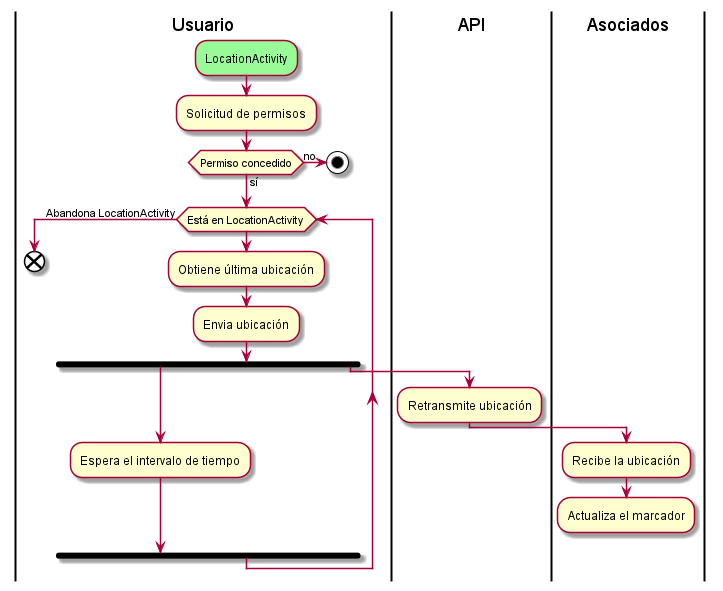
\includegraphics[width=0.5\textwidth]{images/Diseño/ActividadesUbicacion.png}
    \caption{Diagrama de actividades de la difusión de localizaciones}
    \label{dia:actividad_ubicacion}
\end{figure}

Para poder compartir la ubicación del usuario es necesario que este \textbf{conceda permisos} a la aplicación para poder usar los servicios de su dispositivo que la proporcionan. Una vez que lo haga, la aplicación mostrará al usuario una pantalla con un mapa y su localización además de la del resto de usuarios conectados, si hay alguno. En ese momento también se iniciará una tarea de fondo que de forma repetida tras un intervalo de tiempo \textbf{solicitará la última ubicación} del usuario y procederá a enviarla por el WebSocket a la \acrshort{api}.

\begin{figure}[H]
    \centering
    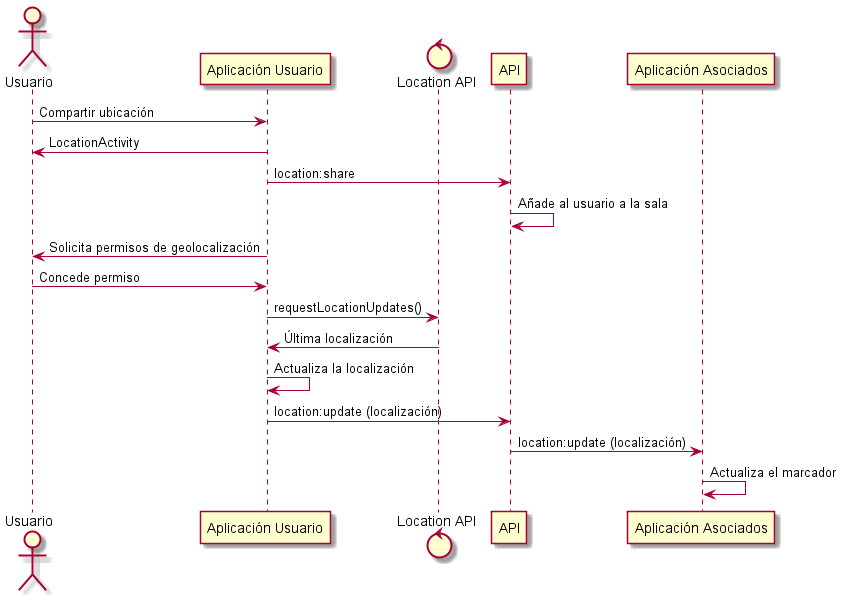
\includegraphics[width=0.7\textwidth]{images/Diseño/SecuenciaUbicacion.png}
    \caption{Diagrama de secuencia de la difusión de localizaciones}
    \label{dia:secuencia_ubicacion}
\end{figure}

La \acrshort{api} recibirá las ubicaciones de los usuario a través del evento de actualización (\fref{ws:location_update}), mismo evento que usará para \textbf{retransmitir esa ubicación} al resto de usuario conectados a dicha sala (pero no al emisor). Los usuarios asociados que estén compartiendo su ubicación recibirán la ubicación del usuario a través de dicho evento y actualizarán el marcador del mismo acorde a la nueva localización.